\documentclass[a4paper,11pt]{report}
\usepackage[T1]{fontenc}
\usepackage[utf8]{inputenc}
\usepackage{lmodern}
\usepackage[francais]{babel}
\usepackage[usenames,dvipsnames,svgnames,table]{xcolor}
\usepackage[colorlinks,linkcolor={blue!30!black},citecolor={blue!50!black},urlcolor={blue!80!black}]{hyperref}
\usepackage{amsmath,array,graphicx,caption,lmodern,subcaption,tikz,url,xspace,wrapfig}
\usepackage{textcomp,rotating,epic,eepic,pdfpages}
\usepackage[top=2cm,left=2.5cm,right=2.5cm,bottom=2cm]{geometry} % Géométrie de la page, modifier selon le besoin
\usepackage[babel=true,kerning=true]{microtype}
\usepackage{float}

% \pdfsuppresswarningpagegroup=1
\title{Rapport de Stage d'Application}


\begin{document}
\pagenumbering{gobble}  % Pas de numérotation
\begin{titlepage}
    \vspace*{50px}
    
\includegraphics[height=80px]{Images/logo_phelma.pdf}
    \vspace*{-80px}
\begin{flushright}
%     \vspace*{60px}
    
\includegraphics[height=65px]{Images/CIME.jpg}
\end{flushright}

\vspace*{2cm}

\begin{center}
\rule{\linewidth}{0.5mm}\\[0.4cm]
{\huge{\bfseries Compte Rendu}\\[0.4cm]
\textsc{TP Simulation électronique}\\[0.4cm]}
\rule{\linewidth}{0.5mm}\\[0.5cm]

\LARGE{\textsc{Nicolas Paillet, Félix Piédallu \& Giulia Rizzo}}\\[0.7cm]
\large{\textsc{2015-2016}}\\[2cm]

\Large{~}\\[1cm]
% 
\includegraphics[width=0.4\textwidth]{Images/CIME.jpg}\\[1cm]
%
 \large{Encadrant : Marco Pala}\\[2cm]
%

\end{center}
\end{titlepage}

\tableofcontents        % Table des matières avec liens, générée automatiquement.
\newpage
\pagenumbering{arabic}  % Numérotation de retour !


\chapter{Introduction}
Lors de la conception de composant à semiconducteurs, il est important d'avoir des outils de simulation pour avoir une idée des résultats et performances attendues. Il est également important de maîtriser ces outils de simulation pour réaliser ces simulations. Ce TP a pour but de nous initier à certains de ces outils en nous proposant de réaliser la simulation de composants MOS tel que ceux étudiés de manière théorique en cours. Ainsi, nous pourrons mettre des graphes  numériques sur les équations calculées théoriquement.

\chapter{Architecture "Bulk"}

\section{Position du problème}
Dans cette partie, on cherche à modéliser un transistor dit "Bulk", que l'on peut représenter schématiquement (Figure \ref{SchemaBulk})
\begin{figure}[H]
\centering
\begin{tikzpicture}
\fill [color=gray!20] (3,5)--(7,5)--(7,4.8)--(3,4.8)--cycle;
\fill [color=black] (3,5)--(7,5)--(7,5.2)--(3,5.2)--cycle;
\draw [thick] (0,5)--(10,5);
\draw (3,5)--(3,3)--(0,3);
\draw (1.5,4)node{n};
\draw (7,5)--(7,3)--(10,3);
\draw (8.5,4)node{n};
\draw (5,4.8)node[below]{Canal};

\draw (3,5)--(3,6)--(7,6)--(7,5)--cycle;

\end{tikzpicture}
\caption{Schéma d'un transistor Bulk}
\label{SchemaBulk}
\end{figure}
\section{Initialisation de la simulation}

Tout d'abord, on utilise l'éditeur \texttt{deckbuild} afin de mettre en place la séquence de commandes à réaliser dans le logiciel \texttt{Atlas}. En premier lieu il faut créer un maillage 2D pour pouvoir y inclure des régions.
\vspace{0.3cm}

\noindent\fbox{
\begin{minipage}{\textwidth}
\noindent\texttt{go atlas\\mesh space.mult = 1.0\\x.mesh loc=0.0 spac=0.001\\x.mesh loc=0.1 spac=0.001\\x.mesh loc=0.2 spac=0.001\\x.mesh loc=0.3 spac=0.001\\y.mesh loc=0.000 spac=0.0001\\y.mesh loc=0.002 spac=0.0001\\y.mesh loc=1.002 spac=0.01}
\end{minipage}}
\vspace{0.3cm}

Il faut ensuite dessiner le composant que nous voulons modéliser sur cette grille. Pour cela, il nous suffira de dessiner des régions en précisant les matériaux utilisés pour chacune d'entre elles.
\vspace{0.3cm}

\noindent\fbox{
\begin{minipage}{\textwidth}
\noindent\texttt{region number = 1 x.min=0.0 x.max = 0.3 y.min = 0.0 y.max = 0.002 material = Oxide\\
region number = 2 x.min=0 x.max = 0.3 y.min = 0.002 y.max = 1.002 material = Silicon}
\vspace{0.3cm}

\noindent\texttt{electrode name = gate   number = 1 x.min = 0.1 x.max = 0.2 y.min = 0.00 y.max = 0\\
electrode name = source number = 2 x.min = 0.0 x.max = 0.0 y.min = 0.002 y.max = 0.012\\
electrode name = drain  number = 3 x.min = 0.3 x.max = 0.3 y.min = 0.002 y.max = 0.012}
\vspace{0.3cm}

\noindent\texttt{doping uniform conc = 1E15 p.type region = 2\\
doping uniform conc = 1E20 N.type region = 2 x.left = 0.0 x.right = 0.1 y.max = 0.012\\
doping uniform conc = 1E20 N.type region = 2 x.left = 0.2 x.right = 0.3 y.max = 0.012\\
struct outf = mos.str}
\end{minipage}}
\vspace{0.3cm}

\begin{figure}[H]
\centering
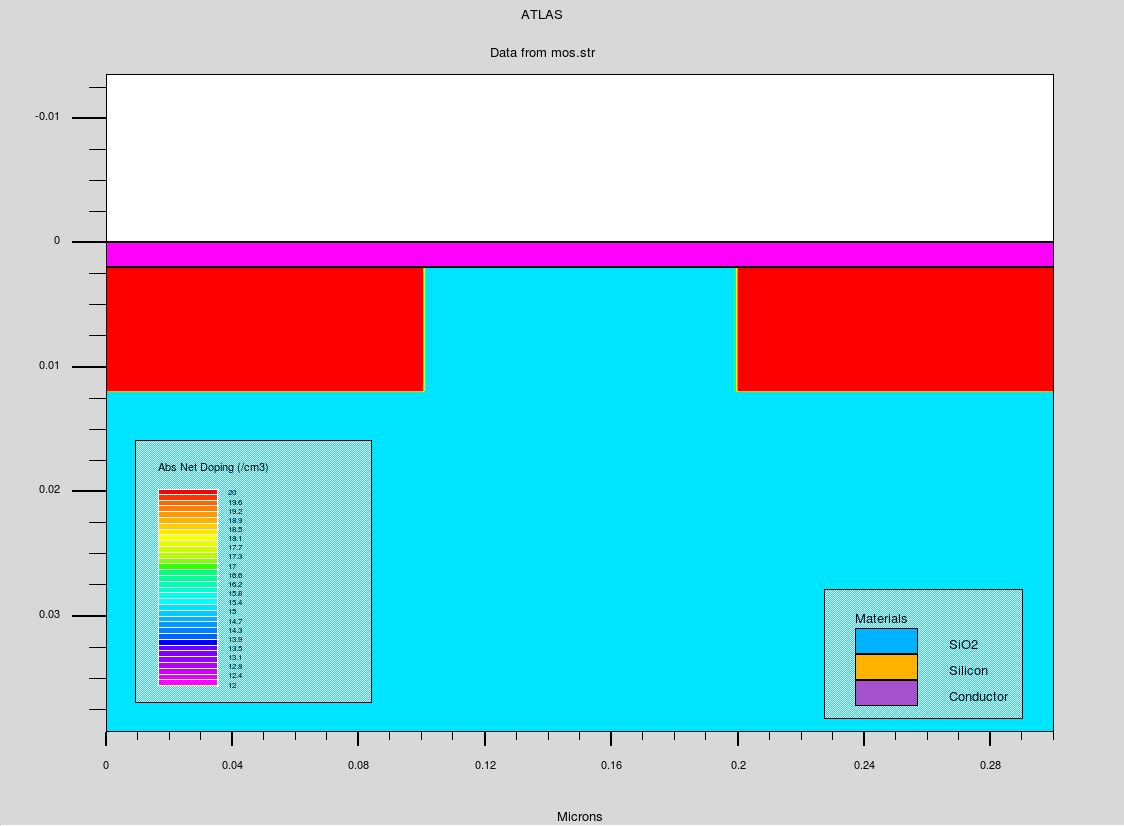
\includegraphics[width=300pt]{Simu1-Dopage.png}
\caption{Image des différentes régions et dopages générés par le logiciel}
\label{transistortonyplot}
\end{figure}

Nous avons ainsi une modélisation 2D du transistor, comme le montre la Figure \ref{transistortonyplot}.

On précise ensuite au logiciel les différents contacts que nous allons utiliser, on obtient ainsi l'image en Figure \ref{TransistorFull}

\begin{figure}[H]
    \centering
    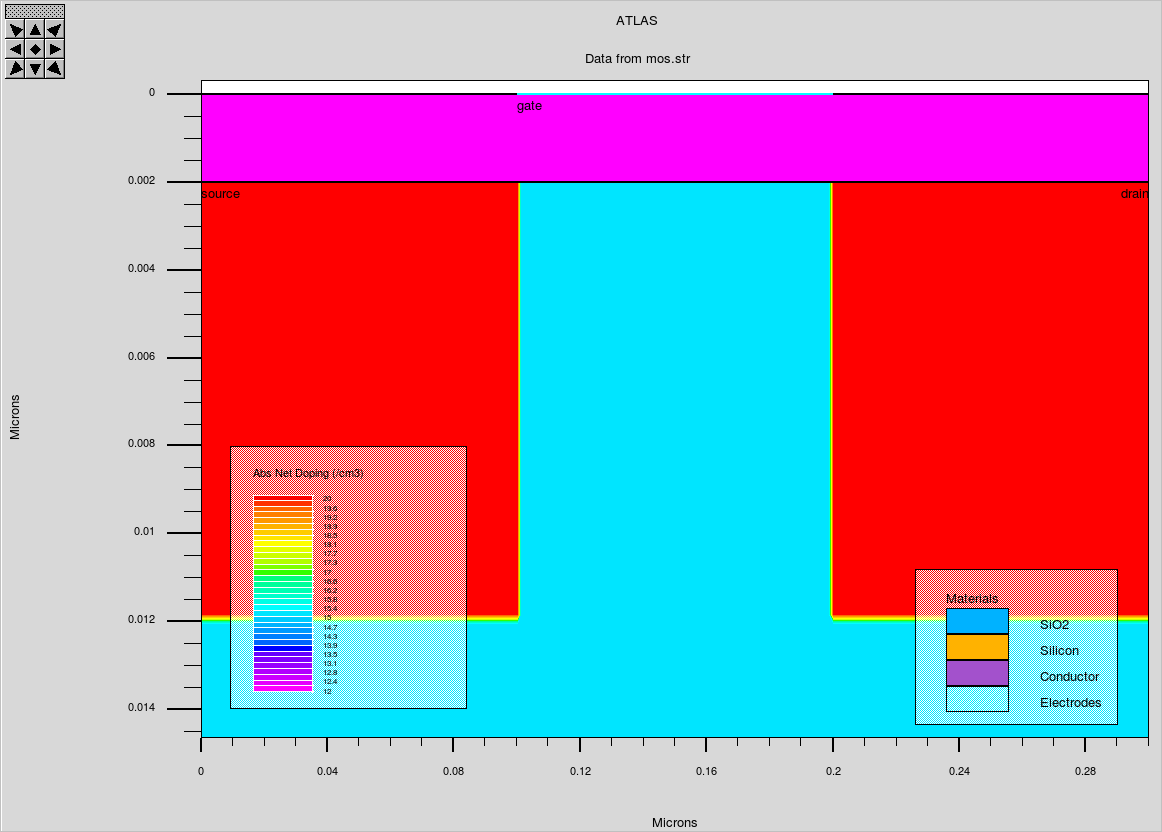
\includegraphics[width=300pt]{TransistorFull.png}
    \caption{Image des régions, du dopage ainsi que des contacts générée par le logiciel}
    \label{TransistorFull}
\end{figure}

Maintenant que notre transistor est modélisé, nous allons pouvoir réaliser des simulations en jouant avec les différentes tensions appliquées.

\section{Tracés de caractéristiques}

En effet, il suffit ensuite d'ajouter quelques lignes au script afin de tracer des courbes, comme le montre la figure \ref{logIdVgmeshfin}.

\noindent\fbox{
\begin{minipage}{\textwidth}
\noindent\texttt{output charge band.param ex.field ey.field jx.tot con.band val.band}
\vspace{0.3cm}

\noindent\texttt{solve init\\
save outfile = nmos1.str}
\vspace{0.3cm}

\noindent\texttt{solve vgate = 0 vdrain = 0 vstep = 0.1 vfinal = 1 name = drain\\
save outfile = nmos2.str}
\vspace{0.3cm}

\noindent\texttt{log outfile = idvg\_vds1.log\\
save outfile = nmos3.str\\
solve vgate = 0 vdrain = 1 vstep = 0.1 vfinal = 2 name = gate\\
extract name="vt" (xintercept(maxslope(curve(abs(v."gate"),abs(i."drain")))) \ }

\hspace{1cm} \texttt{- abs(ave(v."drain"))/2.0)}\\
\texttt{extract name="subvt" \ }

\hspace{1cm} \texttt{ 1.0/slope(maxslope(curve(abs(v."gate"),log10(abs(i."drain")))))}
\end{minipage}}

\begin{figure}[H]
\centering
    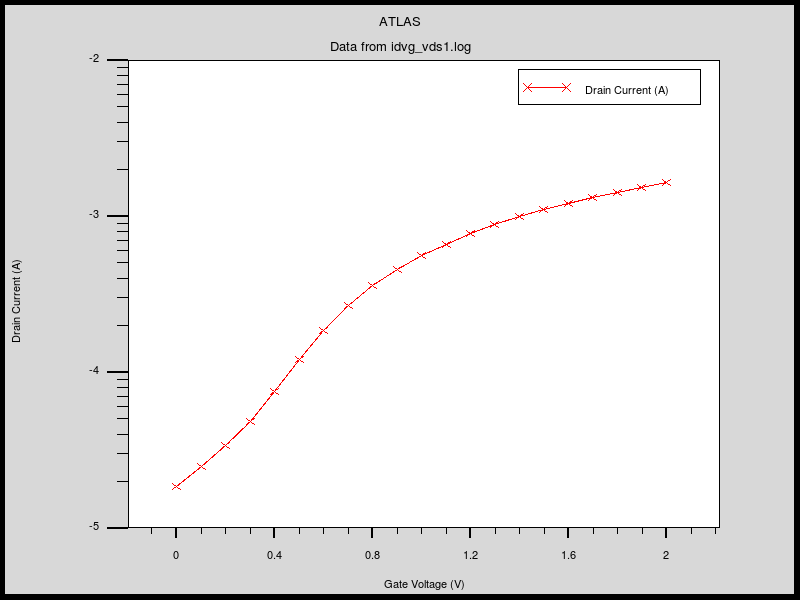
\includegraphics[width=300pt]{Images/MeshFin.png}
    \caption{Caractéristique logarithmique $\log(I_d(V_g))$}
    \label{logIdVgmeshfin}
\end{figure}

A partir de ce graphe il est possible extraire différents paramètres. Par exemple, pour $V_{ds}=50mV$, on trouve $V_t=350mV$ et $SubV_t=170mV/decade$, $I_{sat}=20mA$ et $I_{off}=20\mu A$.

\section{Optimisation du maillage}

Nous avons pu voir lors des calculs précédents qu'avec le maillage proposé initialement, l'obtention de points est très longue. En effet, le maillage est beaucoup trop fin, en particulier à des endroits où il n'a pas besoin de l'être. Par exemple le maillage n'a pas besoin d'être précis loin en profondeur, ni loin des interfaces. Par contre, proche des interfaces il faut qu'il soit fin pour bien représenter les changements brusques.
 
\vspace{0.3cm}

On modifie alors le maillage comme suit :
\vspace{0.3cm}

\noindent\fbox{
\begin{minipage}{\textwidth}
\noindent\texttt{mesh space.mult = 1.0\\
x.mesh loc = 0.0 spac = 0.005\\
x.mesh loc = 0.1 spac = 0.001\\
x.mesh loc = 0.2 spac = 0.001\\
x.mesh loc = 0.3 spac = 0.005\\
y.mesh loc = 0.000 spac = 0.0001\\
y.mesh loc = 0.002 spac = 0.001\\
y.mesh loc = 0.020 spac = 0.01\\
y.mesh loc = 1.002 spac = 0.01}
\end{minipage}}
\vspace{0.3cm}

On peut ainsi également tracer la caractéristique obtenue avec ce maillage, en figure \ref{logIdVgmeshopti}

\begin{figure}[H]
    \centering
    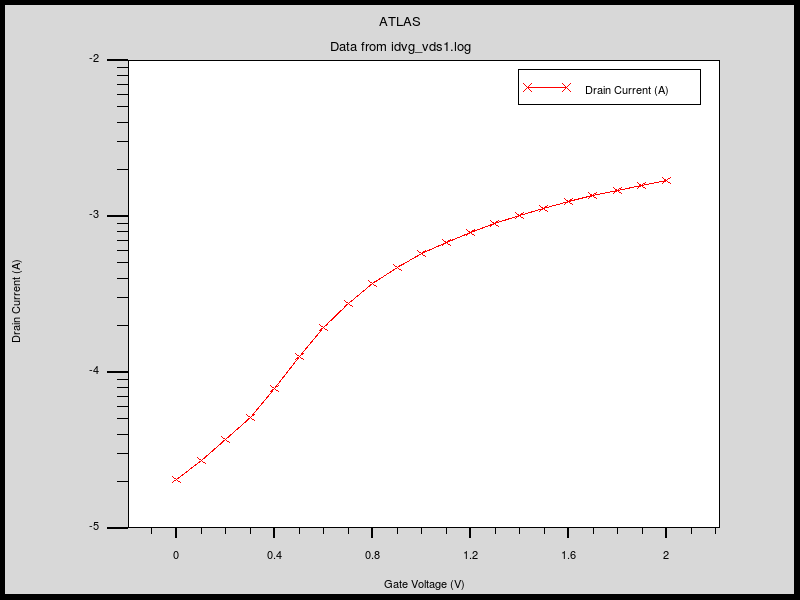
\includegraphics[width=300pt]{../meshOpti1/Log.png}
    \caption{Caractéristique $\log(I_g(V_g))$ obtenue avec un maillage optimisé.}
    \label{logIdVgmeshopti}
\end{figure}

Il convient ensuite de comparer les deux courbes obtenues, pour vérifier si le maillage moins précis donne le même résultat que le maillage fin.


\section{Extraction des paramètres}
A partir des caractéristiques tracées, nous pouvons remonter à certains paramètres. Par exemple, SS et DIBL.



%SS 

%DIBL


\chapter{Une autre architecture : FDSOI}

\section{Position du problème}

On passe à une architecture FDSOI pour limiter les effets de canaux courts.

%schéma

\section{Simulation}
On reprend les élements précedents en rajoutant une zone d'oxyde sous le silicium dopé n.

On obtient ainsi le dispositif suivant :

%image de dispo


\section{Tracé des caractéristiques}

On peut ainsi tracer les caractéristiques :
\begin{figure}[H]
    \centering
    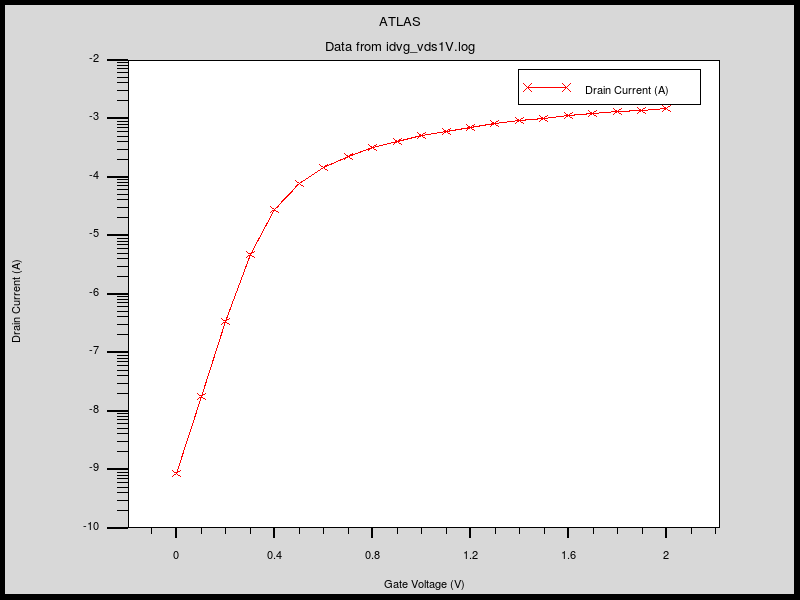
\includegraphics[width=300pt]{../FDSOI/LogIdVg.png}
    \caption{Caractéristiques $\log(I_d(V_g))$ pour $V_d$ faible (en rouge) et $V_d$ fort (en vert)}    
\end{figure}


\section{Extraction des paramètres}

De même qu'avec l'architecture précédente, on peut extraire les paramètres SS et DIBL.

%SS

%DIBL
\chapter{Architecture Bulk}



\chapter{Longueur de grille}

\section{Comparaison des caractéristiques}

\section{Evolution de $V_T$}

\section{}



\end{document}
